% Gemini theme
% https://github.com/anishathalye/gemini

\documentclass[20pt, final]{beamer}

% ====================
% Packages
% ====================

%\usepackage[T1]{fontenc}
\usepackage{lmodern}
\usepackage[size=a1, scale=1.0, orientation=portrait]{beamerposter}
\usetheme{gemini}
\usecolortheme{gemini}
\setbeamerfont{block body}{family=\Lato,size={\fontsize{18}{20}}}
\setbeamerfont{enumerate item}{size={\fontsize{18}{20}}}

\usepackage{graphicx}
\usepackage{booktabs}
\usepackage{tikz}
\usetikzlibrary{quantikz}
\usepackage{pgfplots}
\definecolor{amethyst}{rgb}{0.6, 0.33, 0.73}
\usepackage{fontawesome}
\pgfplotsset{compat=1.14}
\usepackage{anyfontsize}
\usepackage{tcolorbox}
\usepackage{wrapfig}
\usepackage{braket}
\usepackage{bm}

\usepackage{xspace,slashed}
\usepackage{algorithm2e}
\SetKwComment{Comment}{/* }{ */}


%% ---------- useful for the schema ---------

\usetikzlibrary{positioning,arrows,calc,math,angles,quotes}
\usetikzlibrary{arrows,automata}
\usetikzlibrary{positioning}
\usetikzlibrary{arrows.meta,
                bending,
                intersections,
                quotes,
                shapes.geometric}

\tikzset{
    state/.style={
           rectangle,
           rounded corners,
           draw=black, very thick,
           minimum height=1em,
           inner sep=2pt,
           text centered,
           },
}



\definecolor{darkmidnightblue}{rgb}{0.0, 0.2, 0.4}

% ====================
% Lengths
% ====================

% If you have N columns, choose \sepwidth and \colwidth such that
% (N+1)*\sepwidth + N*\colwidth = \paperwidth
\newlength{\sepwidth}
\newlength{\colwidth}
\setlength{\sepwidth}{0.025\paperwidth}
\setlength{\colwidth}{0.42\paperwidth}


% useful for the logos

\logoright{
\includegraphics[height=4cm]{figures/qr-code.png}}
\logoleft{
\includegraphics[height=4cm]{figures/qibo_qr.png}}

\newcommand{\separatorcolumn}{\begin{column}{\sepwidth}\end{column}}

% ====================
% Title
% ====================

\title{Real-time error mitigation for variational optimization on quantum hardware}

\author{Alejandro Sopena\inst{1}, Matteo Robbiati\inst{2  }\inst{3}, Andrea Papaluca\inst{4  }\inst{5} and Stefano Carrazza\inst{2  }\inst{3  }\inst{5  }}


\institute[shortinst]{
  \inst{2  } TIF Lab, Dipartimento di Fisica, Universit\`a degli Studi
  di Milano, Milan, Italy. 

  \inst{3  } CERN, Theoretical Physics Department, CH-1211
  Geneva 23, Switzerland.

  \inst{1  } Instituto de F\'{\i}sica Te\'{o}rica, UAM/CSIC, Universidad Aut\'{o}noma de Madrid, Cantoblanco, Madrid, Spain

  \inst{4  } School of Computing, The Australian National University, Canberra, ACT, Australia.

  \inst{5  } Quantum Research Center, Technology Innovation Institute, Abu Dhabi, UAE.
  }

% ====================
% Footer (optional)
% ====================

\footercontent{
  
\includegraphics[height=2cm]{figures/qibo_logo.png} \qquad \qquad \qquad \,\,\,
  
\includegraphics[height=2cm]{figures/unimi.jpg} \qquad \qquad \qquad \,\,\,
  
\includegraphics[height=2cm]{figures/ift.eps} \qquad \qquad \qquad \,\,\,
  
\includegraphics[height=2cm]{figures/qti.png} \qquad \qquad \qquad \,\,\,
  
\includegraphics[height=2cm]{figures/anu-logo.png} \qquad \qquad \qquad \,\,\,
 
\includegraphics[height=2cm]{figures/tii-logo-dark.eps} \qquad \qquad \qquad \,\,\,
  
\includegraphics[height=2cm]{figures/cern.jpg} 
  \hfill
}
% (can be left out to remove footer)

% ====================
% Logo (optional)
% ====================

% use this to include logos on the left and/or right side of the header:
% \logoright{\includegraphics[height=7cm]{logo1.pdf}}
% \logoleft{\includegraphics[height=7cm]{logo2.pdf}}

% ====================
% Body
% ====================

\begin{document}

\begin{frame}[t]
\begin{columns}[t]
\separatorcolumn


\begin{column}{\colwidth}

\begin{alertblock}{Aim}
We put forward the inclusion of error mitigation routines in the process of training
Variational Quantum Circuit (VQC) models. In detail, we define a Real Time Quantum 
Error Mitigation (RTQEM) algorithm to coadiuvate the task of fitting functions 
on quantum chips with VQCs.
\end{alertblock}

\begin{block}{Schematic pipeline of the RTQEM algorithm}
    \begin{figure}
    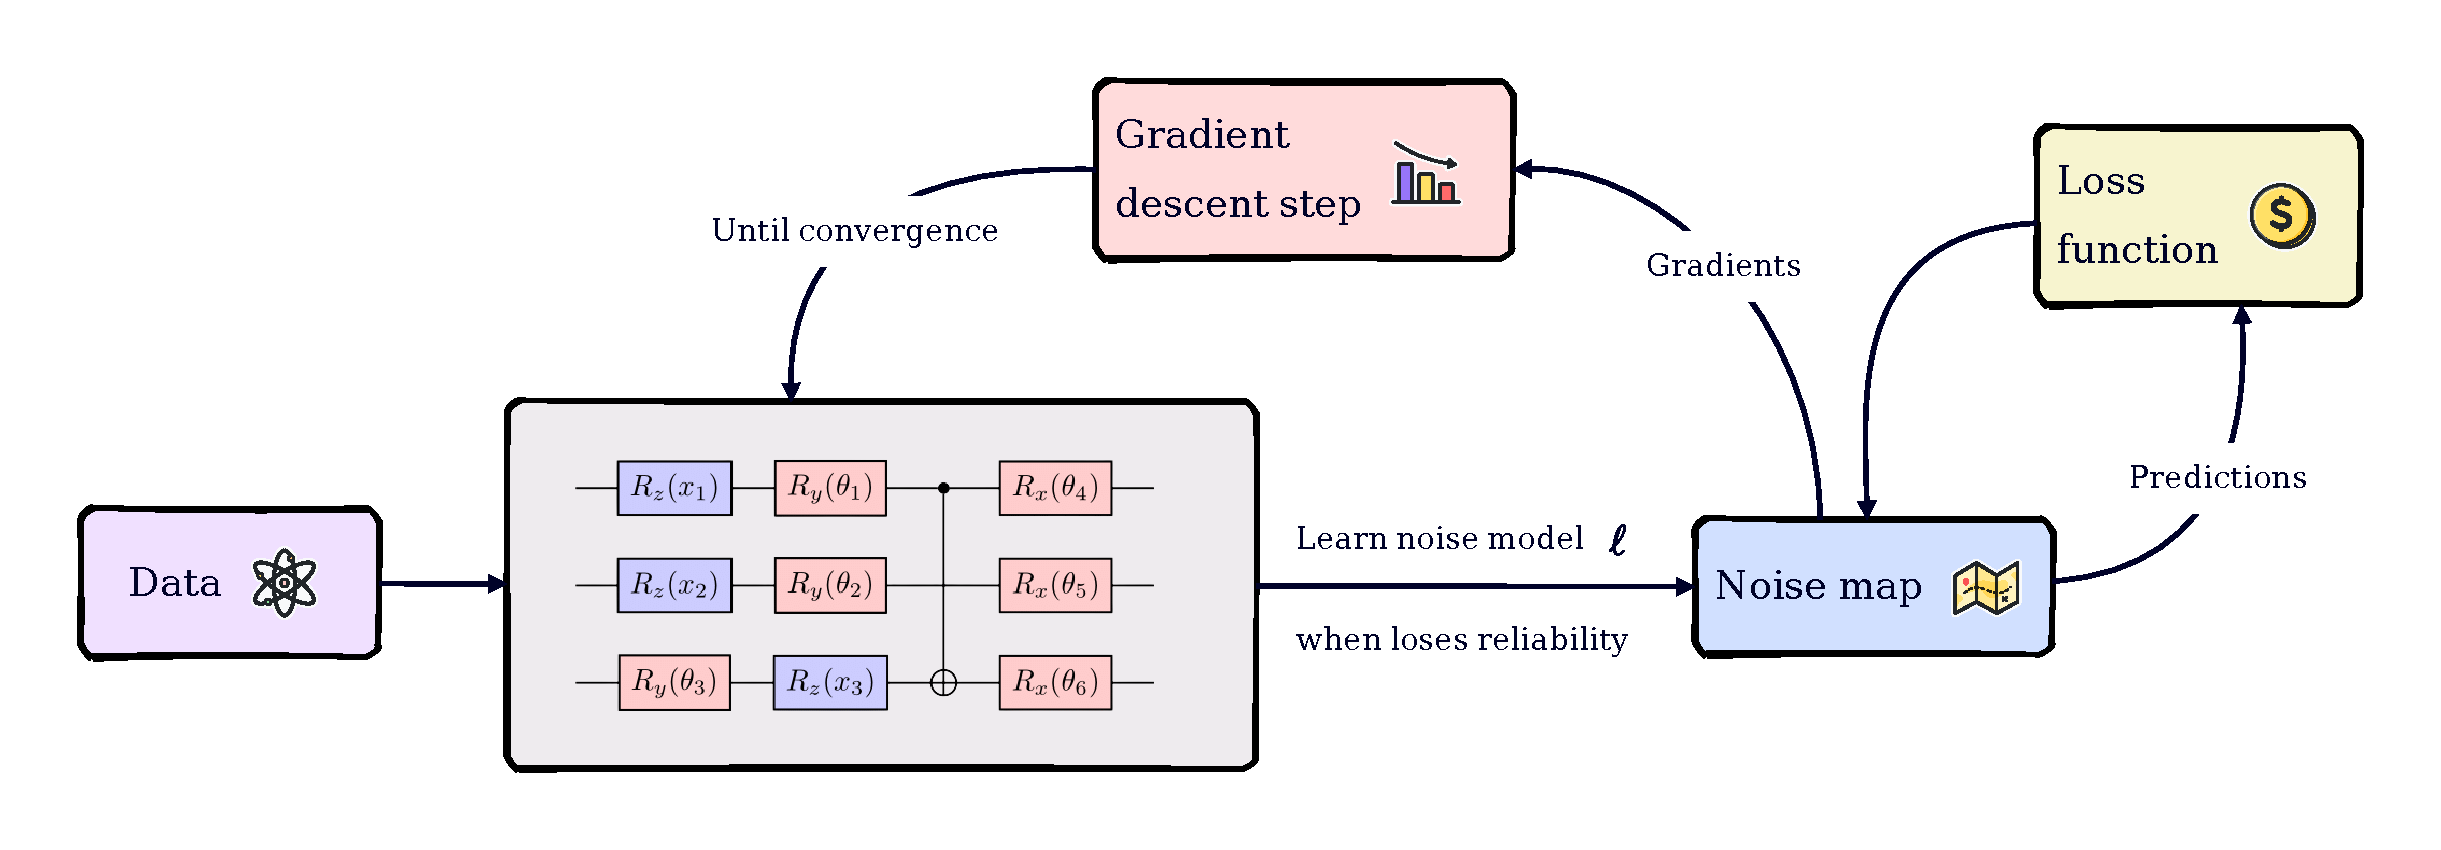
\includegraphics[width=1\textwidth]{figures/rtqem.pdf}%
    \end{figure}
\end{block}

\begin{alertblock}{Ansatz}
We tackle multi-dimensional regression problems using a VQC as Quantum Machine Learning (QML)
model. The data $\bm{x}$ are encoded into the circuit via Data Reuploading~\cite{reuploading},

\begin{figure} 
  \begin{tikzcd}[row sep = 2]
  \lstick{$\ket{0}$} & \gate{L(x_1| \bm{\theta}_{1,1})} & \ctrl{1} & \qw       & \qw       & \qw      & \targ{}   &   \qw & \ \cdots \ & \gate{L(x_1| \bm{\theta}_{N_{\rm layers},1})} & \ctrl{1} & \qw       & \qw       & \qw      & \targ{} & \meter{} \\
  \lstick{$\ket{0}$} & \gate{L(x_2| \bm{\theta}_{1,2})} & \targ{}  & \ctrl{1}  & \qw       & \qw      & \qw       &   \qw & \ \cdots \ & \gate{L(x_2| \bm{\theta}_{N_{\rm layers},2})} & \targ{}  & \ctrl{1}  & \qw       & \qw      & \qw & \meter{}  \\
  \lstick{$\ket{0}$} & \gate{L(x_3| \bm{\theta}_{1,3})} & \qw      & \targ{}   & \ctrl{1}  & \qw      & \qw       &   \qw & \ \cdots \ & \gate{L(x_3| \bm{\theta}_{N_{\rm layers},3})} & \qw      & \targ{}   & \ctrl{1}  & \qw      & \qw & \meter{} \\
  \lstick{$\ket{0}$} & \gate{L(x_4| \bm{\theta}_{1,4})} & \qw      & \qw       & \targ{}   & \ctrl{1} & \qw       &   \qw & \ \cdots \ & \gate{L(x_4| \bm{\theta}_{N_{\rm layers},4})} & \qw      & \qw       & \targ{}   & \ctrl{1} & \qw & \meter{} \\
  \lstick{$\ket{0}$} & \gate{L(x_n| \bm{\theta}_{1,n})} & \qw      & \qw       & \qw       & \targ{}  & \ctrl{-4} &   \qw & \ \cdots \ & \gate{L(x_n| \bm{\theta}_{N_{\rm layers},n})} & \qw      & \qw       & \qw       & \targ{}  & \ctrl{-4} & \meter{} \\ 
  \end{tikzcd}
\label{fig:qpdf}
\end{figure}

with the following definition of the uploading channel:
\begin{equation}
L(x_j| \bm{\theta}_{l,j}) = R_z(\theta_3\,x_j + \theta_4) R_y(\theta_1\, \kappa(x_j) + \theta_2) \ ,
\label{eq:uploading_layer}
\end{equation}
which uploads the $j$-th component of $\bm{x}$ at the circuit layer $l$.
\end{alertblock}

\begin{block}{Noise of a quantum hardware}
We consider a quantum system affected by local pauli noise with parameters 
$-1 \leq q_X, q_Y, q_Z \leq +1$ and readout noise parametrized by bit-flip probability 
$(1-q_M)/2$. This setup gives rise to Noise-Induced Barren Plateaus (NIBP)~\cite{nibp}, which tend 
to concentrate the expectation value around 0. 
    \begin{figure}
    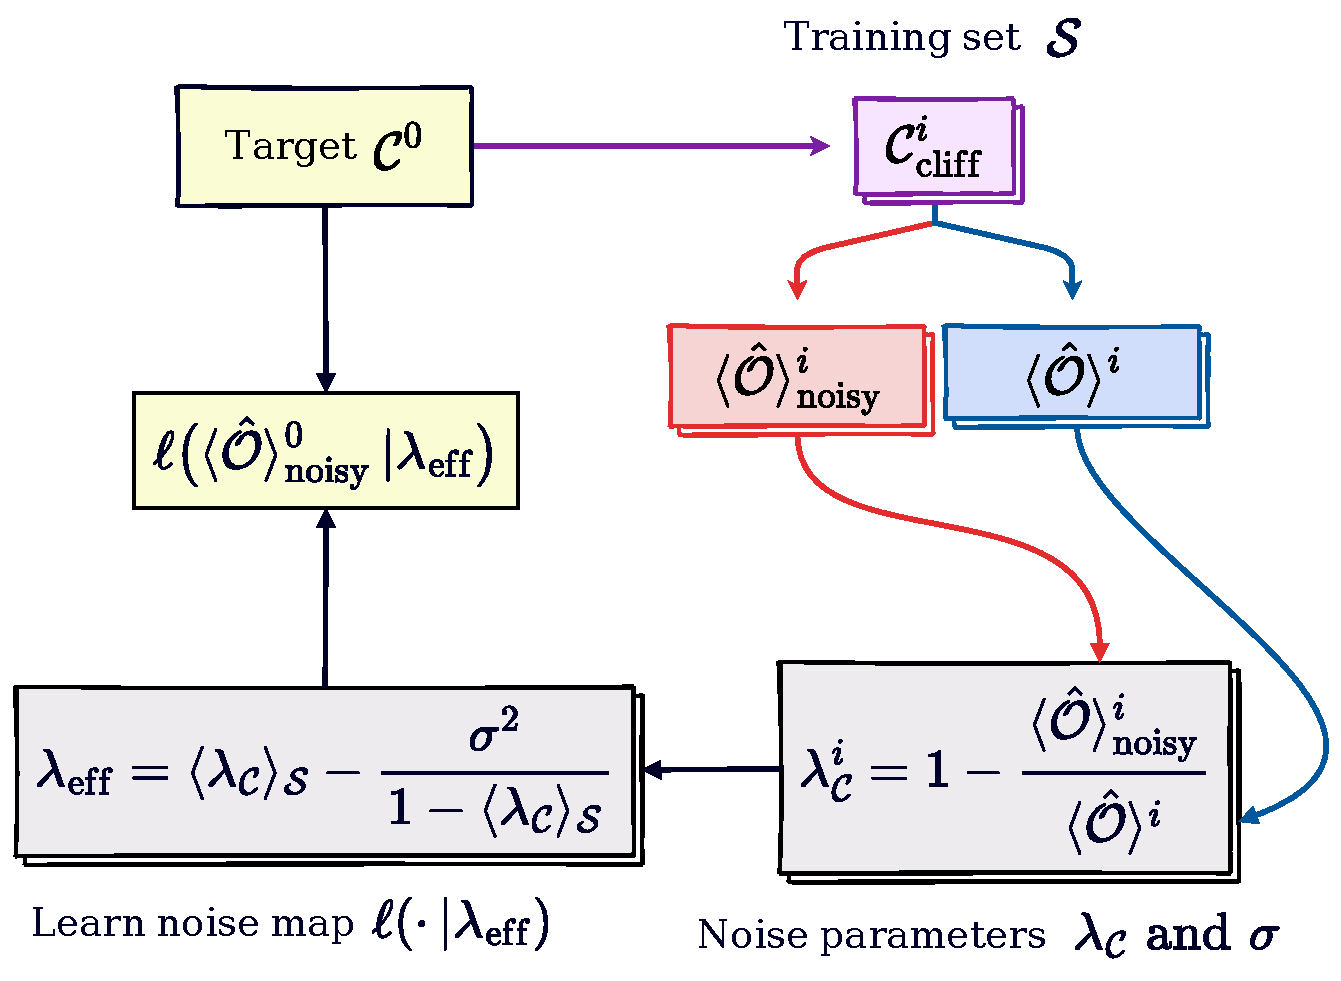
\includegraphics[width=0.65\textwidth]{figures/ics.pdf}%
    \end{figure}
To mitigate the effect of the noise, we use the Importance Clifford Sampling (ICS)~\cite{ics}
technique, which is a learning-based method which can be used to learn a noise 
map $\ell$ using a training set of Clifford circuits $\mathcal{S}=\{\mathcal{C}^i_{\rm cliff}\}$
built on top of the target circuit $\mathcal{C}^0$.
\end{block}

\begin{block}{Simulation $1$-dim:  $u$-quark PDF}
We firstly use a single-qubit circuit to fit the $u$-quark Parton Distribution 
Function (PDF). We set $q_M=0.005$, $q_X=0.007$, $q_Y=0.003$ and $q_Z=0.002$.
We compare four configurations: noiseless, noisy unmitigated, noisy with mitigation on 
the final predictions (fQEM) and noisy trained with RTQEM. 
\begin{figure}
  \centering
    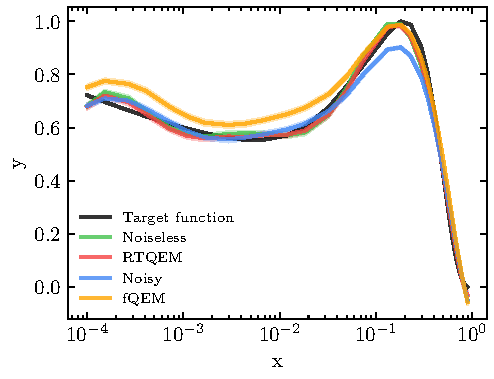
\includegraphics[width=0.5\linewidth]{figures/qpdf.pdf}%
    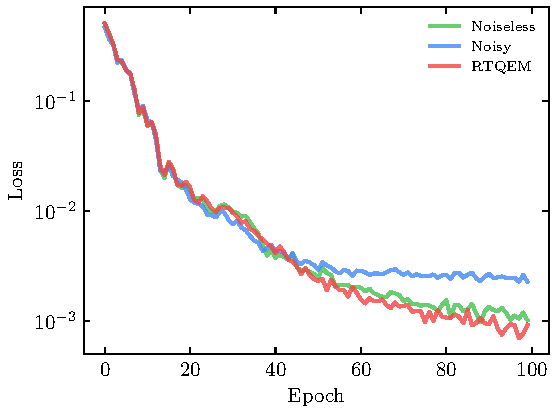
\includegraphics[width=0.5\linewidth]{figures/qpdf_loss.pdf}
    \label{fig:qpdf_simulation}
  \end{figure}
\end{block}

\end{column}

\begin{column}{\colwidth}

\begin{block}{Simulation $n$-dim}
We then tackle a simple multi dimensional target to scale up with the number of 
qubits.
\begin{figure}
  \centering
    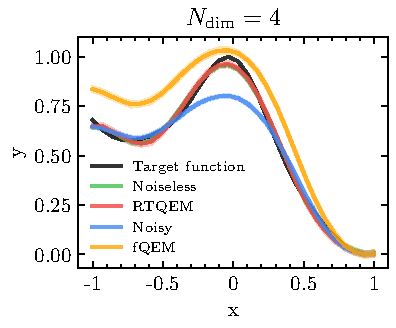
\includegraphics[width=0.33\linewidth]{figures/cos4d.pdf}%
    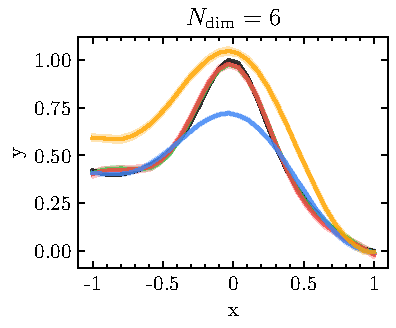
\includegraphics[width=0.33\linewidth]{figures/cos6d.pdf}%
    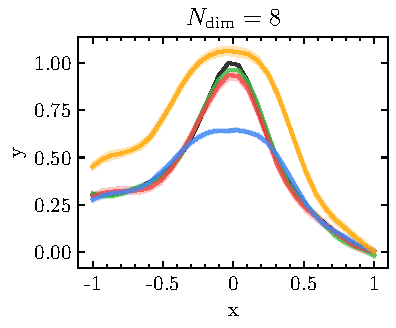
\includegraphics[width=0.33\linewidth]{figures/cos8d.pdf}
    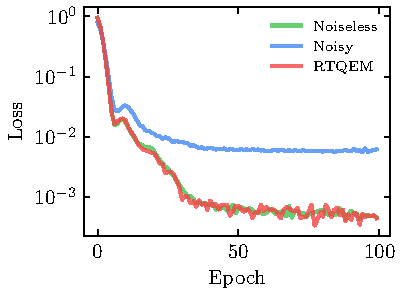
\includegraphics[width=0.33\linewidth]{figures/cos4d_loss.pdf}%
    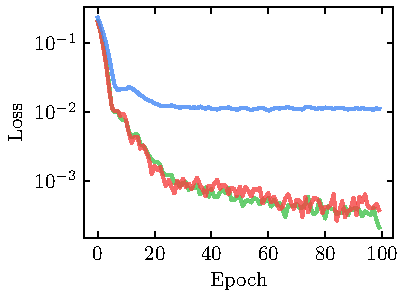
\includegraphics[width=0.33\linewidth]{figures/cos6d_loss.pdf}%
    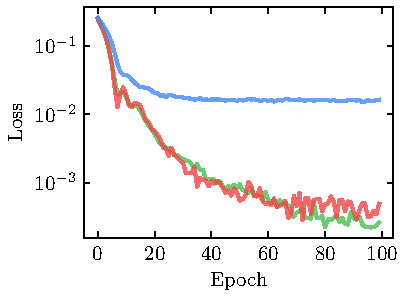
\includegraphics[width=0.33\linewidth]{figures/cos8d_loss.pdf}
    \label{fig:ndim_simulation}
  \end{figure}
\end{block}

\begin{alertblock}{Simulation results}
Mean squared error between the target labels and the predicted values.
\begin{center}
\begin{tabular}{ccccc}
\hline \hline 
\textbf{Target} & $\text{MSE}_{\rm noiseless}$ & $\text{MSE}_{\rm noisy}$ & $\text{MSE}_{\rm fqem}$ & $\text{MSE}_{\rm rtqem}$\\
\hline
$u$ PDF    &  $0.008$  & $0.018$  & $0.023$ & $0.008$ \\
$\cos 4$d  &  $0.003$  & $0.043$  & $0.140$ & $0.003$ \\
$\cos 6$d  &  $0.002$  & $0.083$  & $0.214$ & $0.002$ \\
$\cos 8$d  &  $0.001$  & $0.118$  & $0.360$ & $0.004$ \\
\hline \hline
\end{tabular}
\end{center}
\end{alertblock}

\begin{block}{Evolving noise scenario}
To study how the RTQEM procedure behave in a realistic scenario, we let the noise 
parameters vary following a Random Walk-like evolution.
\begin{figure}
  \centering
    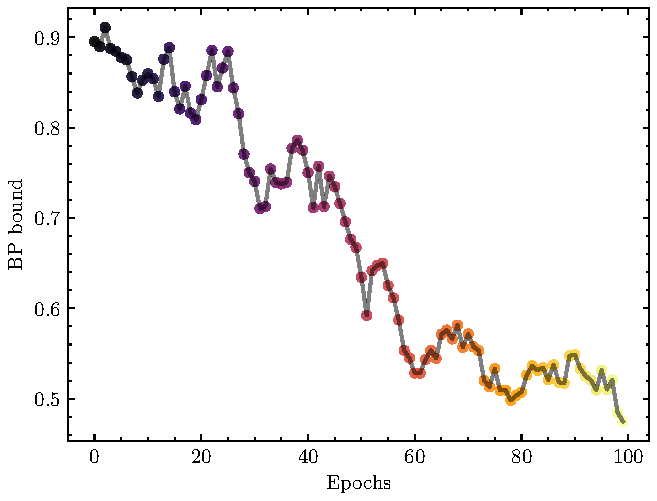
\includegraphics[width=0.49\linewidth]{figures/bound_variation.pdf}%
    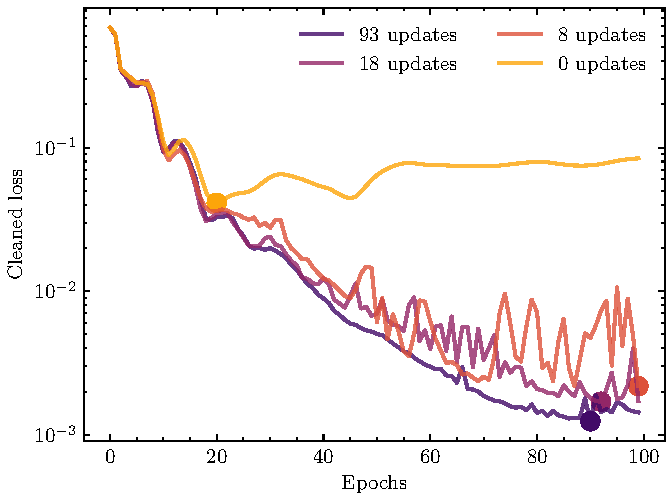
\includegraphics[width=0.5\linewidth]{figures/cleaned_losses.pdf}%
    \label{fig:ndim_simulation}
  \end{figure}
\end{block}



\begin{block}{$u$-quark PDF fit on superconducting devices}
We finally test the RTQEM algorithm on two superconducting devices.
\begin{figure}
  \centering
    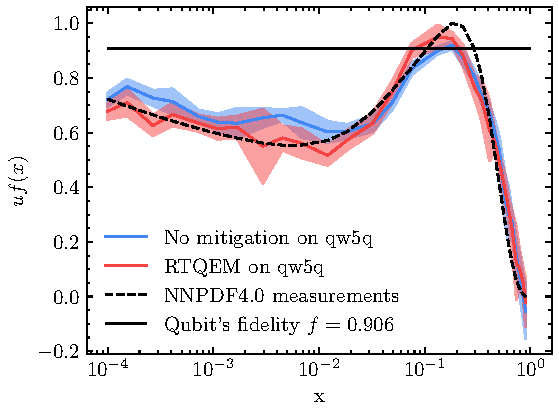
\includegraphics[width=0.5\linewidth]{figures/qw5q_short.pdf}%
    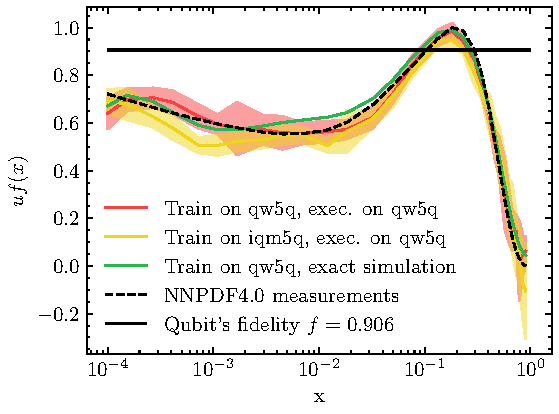
\includegraphics[width=0.5\linewidth]{figures/benchs.pdf}%
    \label{fig:hdw}
  \end{figure}
\end{block}

\begin{alertblock}{Hardware results}
We benchmark the MSE values of various prediction configurations.
\begin{center}
\begin{tabular}{ccccc}
\hline \hline 
\textbf{Training} & \textbf{Predictions} &  \textbf{Config.} & $N_{\rm epochs}$ & MSE \\
\hline
\texttt{qw5q} & \texttt{qw5q} & Noisy & $50$ & $0.0055$   \\     
\texttt{qw5q} & \texttt{qw5q} & RTQEM & $50$ & $0.0042$   \\     
\texttt{qw5q} & \texttt{qw5q} & RTQEM & $100$ & $0.0013$  \\     
\texttt{iqm5q} & \texttt{qw5q} & RTQEM & $100$ & $0.0037$ \\   
\texttt{qw5q} & \texttt{sim} & RTQEM & $100$ & $0.0016$ \\   
\hline \hline
\end{tabular}
\end{center}
\end{alertblock}



\vspace{-1cm}
\begin{block}{References}
  \nocite{*}
    \small  {\bibliographystyle{ieeetr}\bibliography{poster.bib}}
  \end{block}
\end{column}

\separatorcolumn
\end{columns}
\end{frame}

\end{document}
